\documentclass{article}
\usepackage{helvet}
\usepackage{geometry}
\usepackage{graphicx}
\usepackage{amsmath}
\usepackage{hyperref}
\usepackage{xcolor}
\usepackage{titlesec}
\usepackage{microtype} % Prevents overfull hboxes by better text wrapping
\geometry{margin=1in}
\usepackage{subcaption}
\usepackage{listings}
\usepackage{color}
% Define colors for code syntax highlighting
\definecolor{codeblue}{rgb}{0.13, 0.13, 0.7}
\definecolor{codegreen}{rgb}{0, 0.5, 0}
\definecolor{codegray}{rgb}{0.5, 0.5, 0.5}
\definecolor{codepurple}{rgb}{0.58, 0, 0.82}

\lstdefinestyle{mystyle}{
    backgroundcolor=\color{white},   
    commentstyle=\color{codegreen},
    keywordstyle=\color{codeblue},
    numberstyle=\tiny\color{codegray},
    stringstyle=\color{codepurple},
    basicstyle=\ttfamily\footnotesize,
    breaklines=true,                 
    captionpos=b,                    
    keepspaces=true,                 
    numbers=left,                    
    numbersep=5pt,                  
    showspaces=false,                
    showstringspaces=false,
    showtabs=false,                  
    tabsize=2
}

\lstset{style=mystyle}

% Define colors
\definecolor{primary}{RGB}{0, 102, 204} % Blue color
\definecolor{IITBBlue}{RGB}{0, 51, 102} % IIT Bombay's signature blue

\usepackage{cite}
\usepackage{amsmath,amssymb,amsfonts}
\usepackage{algorithmic}
\usepackage{graphicx}
\usepackage{textcomp}
\usepackage{xcolor}
\usepackage{hyperref}
\usepackage{placeins}
\usepackage{graphicx}
\usepackage{subcaption}
\usepackage{physics}




\def\BibTeX{{\rm B\kern-.05em{\sc i\kern-.025em b}\kern-.08em
    T\kern-.1667em\lower.7ex\hbox{E}\kern-.125emX}}


\title{Question 4: Assignment 3: CS 663, Fall 2024}
\author{
\IEEEauthorblockN{
    \begin{tabular}{cccc}
        \begin{minipage}[t]{0.23\textwidth}
            \centering
            Amitesh Shekhar\\
            IIT Bombay\\
            22b0014@iitb.ac.in
        \end{minipage} & 
        \begin{minipage}[t]{0.23\textwidth}
            \centering
            Anupam Rawat\\
            IIT Bombay\\
            22b3982@iitb.ac.in
        \end{minipage} & 
        \begin{minipage}[t]{0.23\textwidth}
            \centering
            Toshan Achintya Golla\\
            IIT Bombay\\
            22b2234@iitb.ac.in
        \end{minipage} \\
        \\ 
    \end{tabular}
}
}

\date{September 24, 2024}


\usepackage{amsmath}
\usepackage{amssymb}
\usepackage{hyperref}
\usepackage{ulem,graphicx}
\usepackage[margin=0.5in]{geometry}

\begin{document}
\maketitle

\\

\begin{enumerate}
\item 
Consider a 201 × 201 image whose pixels are all black except for the central column (i.e. column index 101
beginning from 1 to 201) in which all pixels have the value 255. Derive the Fourier transform of this image
analytically, and also plot the logarithm of its Fourier magnitude using fft2 and fftshift in MATLAB. Use
appropriate colorbars. \textsf{[8+2=10 points]}
\\
    \makebox[0pt][l]{\hspace{-7pt}\textit{Soln:}} % Aligns "Answer:" to the left
\\
The image, where all pixel values are black except for the central column i.e. 101st column, whose values are all white.
\[
\begin{bmatrix}
0 & 0 & 0 & \cdots & 255 & \cdots & 0 & 0 & 0 \\
0 & 0 & 0 & \cdots & 255 & \cdots & 0 & 0 & 0 \\
\vdots & \vdots & \vdots & \ddots & \vdots & \ddots & \vdots & \vdots & \vdots \\
0 & 0 & 0 & \cdots & 255 & \cdots & 0 & 0 & 0 \\
0 & 0 & 0 & \cdots & 255 & \cdots & 0 & 0 & 0
\end{bmatrix}
\]
The Fourier Transform of the image is given as:
\begin{equation}
    F_d(u, v) = \frac{1}{\sqrt{W_1 W_2}} \sum_{y=0}^{W_1-1} \sum_{x=0}^{W_2-1} f(x, y) \exp \left(- j 2 \pi \left( \frac{ux}{W_1} + \frac{vy}{W_2} \right) \right)
\end{equation}

Substituting the image height and width, we get:
\begin{equation}
    F_d(u, v) = \frac{1}{201} \sum_{y=0}^{200} \sum_{x=0}^{200} f(x, y) \exp \left(- j 2 \pi \left( \frac{ux}{201} + \frac{vy}{201} \right) \right)
\end{equation}

Assuming, x represents the columns and y represents the rows. Now, if we're looping through the $y^{th}$ row:
\begin{equation}
    \sum_{x=0}^{200} f(x, y) \exp \left(- j 2 \pi \left( \frac{u\cdot x}{201} + \frac{v\cdot y}{201} \right) \right) = \sum_{x=0}^{99} 0 + 255 \cdot \exp \left(- j 2 \pi \left( \frac{u\cdot 100}{201} + \frac{v\cdot y}{201} \right) \right) + \sum_{x=101}^{200} 0
\end{equation}

Substituting the value of equation (3) in equation (2), we get:
\begin{equation}
    F_d(u, v) = \frac{1}{201} \sum_{y=0}^{200} 255 \cdot \exp \left(- j 2 \pi \left( \frac{u\cdot 100}{201} + \frac{v\cdot y}{201} \right) \right) = \frac{255}{201} \exp \left(- j 2 \pi \left( \frac{u\cdot100}{201}\right) \right) \sum_{y=0}^{200} \exp \left(- j 2 \pi \left( \frac{v\cdot y}{201} \right) \right)
\end{equation}
The summation over the exponentials is like the sum of a Geometric Progression, where 
\begin{equation}
\begin{aligned}
    a_0 &= \exp\left( -j2\pi \left( \frac{v \cdot 0}{201} \right) \right) = 1 \quad & r &= \exp\left( -j2\pi \left( \frac{v}{201} \right) \right)
\end{aligned}
\end{equation}

And since \(r < 1\), except for \(r = 1\) at \(v = 0\), the sum is given by,
\begin{equation}
\begin{aligned}
S_n &= \frac{1 - \exp\left( -j2\pi \left( \frac{vn}{201} \right) \right)}{1 - \exp\left( -j2\pi \left( \frac{v}{201} \right) \right)}, \quad \text{for} \quad r \neq 1 \\
S_n &= a_0 \cdot n = n, \quad \text{for} \quad r = 1
\end{aligned}
\end{equation}

Thus, the discrete Fourier transform of the image becomes:
\begin{equation}
\begin{aligned}
    F_d(u, v) = \frac{255}{201} \exp \left(- j 2 \pi \left( \frac{u\cdot100}{201}\right) \right) \frac{1 - \exp\left( -j2\pi \left( \frac{v}{1} \right) \right)}{1 - \exp\left( -j2\pi \left( \frac{v}{201} \right) \right)}, \quad \text{for} \quad v \neq 0 \\
    F_d(u, v) = \frac{255}{201} \exp \left(- j 2 \pi \left( \frac{u\cdot101}{201}\right) \right) \cdot 201 = 255 \cdot \exp \left(- j 2 \pi \left( \frac{u\cdot101}{201}\right) \right), \quad \text{for} \quad v = 0
\end{aligned}
\end{equation}
\\ 
\textbf{Plot of the logarithm of the Fourier Magnitude of this image is given by}:

\begin{figure}[!h]
    \centering
    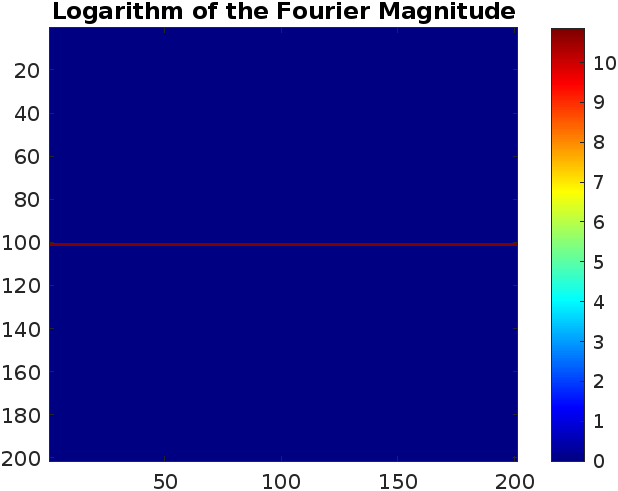
\includegraphics[width=0.5\linewidth]{HomeWork_3/Question_4/images/Q4_fft.png}
    \caption{FT of given image}
\end{figure}
The \textbf{MATLAB code} for the Fourier transform of above image is attached as well as mentioned in the report below.

\begin{lstlisting}[language=matlab]
image = zeros(201, 201);
image(:, 101) = 255;

F = fft2(image);

F_shifted = fftshift(F);

log_magnitude = log(abs(F_shifted) + 1);

figure;
imagesc(log_magnitude);
colormap('jet');
colorbar;
title('Logarithm of the Fourier Magnitude');
\end{lstlisting}
\end{enumerate}
\end{document}
